
\section{Map-Erkennung [H]}
Nachdem der Spieler der Lobby beigetreten ist, wird es Zeit für ihn die Spielumgebung zu zeichnen und diese für die
Abstimmung freizugeben. Das passiert, indem dieser einen QR-Code (``Quick Response''), welcher sich in der
Mitte der Lobby befindet, mit einem mobilen Endgerät, welches über eine Kamera verfügt, abscannt. Somit wird
er auf eine Webseite geleitet, welche wieder auf die Kamera zugreift. Auf dieser ist bereits eine Objekterkennung
vorprogrammiert. Auf die Funktionsweise und auf die technische Umsetzung wird im folgenden \dots eingegangen. Wenn der Spieler
merkt, dass die Objekterkennung das Blatt erkannt hat, kann dieser ein Bild aufnehmen. Im nächsten Schritt ist es nochmals möglich
die erkannten Kanten zu verschieben. Wenn sich der User für das Foto als Map entscheidet, so kann er den ausgewählten Teil in eine
top-down-2d-Perspektive
umwandeln. Kurzgesagt werden dabei die vier ausgewählten Ecken, welche über die Kanten des Blatt Papiers liegen,
für eine Perspektiven-Transformation
mit OpenCV2 herangezogen. Wenn der Spieler dann so weit ist, kann er dieses Bild beziehungsweise diese Map bestätigen und
sendet sie somit zurück an die Lobby. Dann kann die Abstimmung beginnen.

\begin{figure}[H]
    \centering
    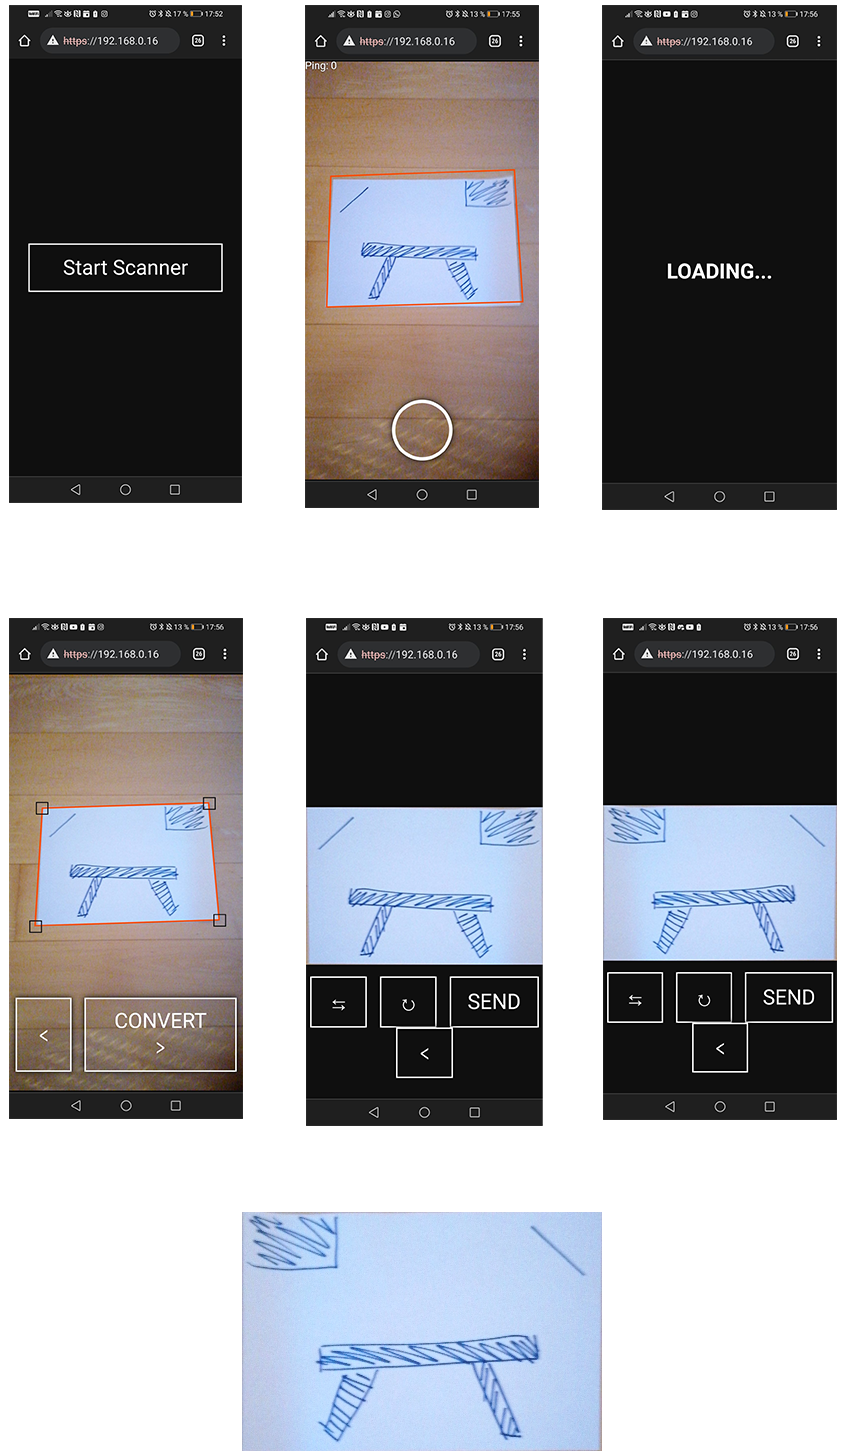
\includegraphics[scale=0.4]{pics/demo_maperkennung/sammlung_1.png}
    \caption{Screenshots der Maperkennungsanwenung}
    \label{fig:map:maperkennungsprozess}
\end{figure}

\setauthor{Himmetsberger Jonas}
\subsection{Objekterkennung [H]}
Das Thema ``Objekterkennung'' ist ein extrem schnell wachsendes und sich verbesserndes Feld in der Welt der Bildverarbeitung beziehungsweise
Bildanalyse. \\
Die Objekterkennung ist ein großer Teil unserer Arbeit. Hier wird aus dem live Footage der Kamera das Blatt Papier und anschließend
in einer fertigen Aufnahme die Map erkannt.
\\
\\
Die Objekterkennung wird zum Beispiel bei komplexen und großen Paketdiensten eingesetzt. Sollen Pakete nach Farbe gruppiert werden, so
reicht bereits ein Farbsensor. Das ist in den meisten Fällen jedoch nicht genügend.
Vielmals werden Pakete auf Strichcodes oder Adressen überprüft.
Wenn also unterschieden werden muss, wo welches Paket landen soll, so ist eine Kamera nötig. Diese muss
ein genügend gut auflösendes Bild aufnehmen, dass daraus Informationen gewonnen werden können. Diese Daten müssen zur Auswertung
mathematisch beschrieben werden. Zur Übersetzung werden Verfahren, wie Kantenerkennung, Transformationen oder Größen- und Farberkennung,
aber auch künstliche Intelligenzen
eingesetzt. In dieser Arbeit wurden Kanten zur Objekterkennung herangezogen.
Die Korrektheit des Ergebnisses ist abhängig von der Korrektheit der bereitgestellten Daten und wie genau das Objekt mathematisch
beschrieben werden kann.
\\
Ein weiteres Beispiel, wo Objekterkennung eingesetzt wird, ist in
Fahrerassistenzsysteme oder autonomes Fahren. Bereits in der ersten Stufe des autonomen Fahrens (dem assistierten Fahren)
werden zur Hilfe Kameras außerhalb des Fahrzeugs angebracht. In einem Auto, welches als Stufe eins autonomes Assistenzsystem
eingestuft wird, werden diese Kameras für einen automatischen Spurhalteassistenten eingesetzt. Via Bildanalyse und Objekterkennung
werden die Linien auf der Straße erkannt. \\
In höheren Stufen ist die Objekterkennung nicht mehr wegzudenken. Es müssen Verkehrsschilder und Personen auf der Straße erkannt
werden um daraufhin entsprechen zu agieren.

Andere Beispiele:
\begin{compactitem}
    \item Gesichtserkennung, um das Smartphone zu entsperren.
    \item Qualitätskontrolle, zur Erkennung und automatischen Entfernung von kaputten oder beschädigten Teilen.
    \item Personenerkennung, um Menschenmassen zu analysieren.
\end{compactitem}

\subsubsection{Beschreibung der Funktionalität [H]}

Wie schon erwähnt kann man aus Bildern Daten erkennen. Viele Pixel bilden insgesamt ein Bild, welches wir visuell aufnehmen und in welchem wir alles Mögliche erkennen können. Jeder einzelne dieser Pixel in einem digitalen Bild enthält Informationen über die Helligkeit und über die Farbe. Der Bildpunkt setzt sich zusammen aus den Farben Rot, Grün und Blau. Aus diesen drei können alle möglichen Farben abgebildet werden.
\\
Bevor ich darauf eingehe, wieso wir uns für die Konturenerkennung als Art der Bilderkennung entschieden haben, ist es noch entscheidend zu wissen, wie der Mensch Objekte erkennt.
\\
In unserem Auge passiert die Farberkennung via den Zapfen. Auch hier wird die Wellenlänge des Lichts in ein Gemisch aus Rot, Grün und Blau aufgeteilt. Allerdings benötigen wir das reine Farbsehen nicht um Objekte zu erkennen. Uns reicht es schon, wenn wir nur Informationen über die Helligkeit empfinden. Somit können wir zum Beispiel auch in Schwarz-Weiß-Bildern oder in der Dunkelheit bei wenig Licht Objekte erkennen. Wir erkennen einen Unterschied zwischen Objekten, welche sich in einem dreidimensionalen Raum befinden leicht, indem das eine Objekt sich in der Helligkeit von dem anderen Objekt unterscheidet. Das heißt, dass wenn z.B. ein Würfel auf einem Boden liegt, dann erkennen wir den Würfel, weil dieser anders viel Licht reflektiert als der Boden. Und an der Stelle, wo der Würfel aufhört, erkennen wir eine Kontur. Hier ist der Unterschied zwischen Boden und Würfel erkennbar.
\\
Und genau so passiert auch die Objekterkennung in unserem Spiel ScribbleFight. Hier wird zuerst aus der Live-View, welche vom Client zur Verfügung gestellt wird, das Farbbild in Graustufen konvertiert. Das passiert, indem für jeden Pixel ein ``Durchschnitts-Wert'' der Helligkeit von allen drei Farbwerte (Rot, Grün, Blau), welche in einem 8-Bit System von 0 bis 255 geht, gebildet wird. Wie dies jedoch genauer funktioniert, wird im Kapitel Bildverarbeitungsalgorithmen
\ref{maai:alogs}
genauer erklärt.

\begin{lstlisting}[caption=Alle unnötigen Bilddaten entfernen,language=Python,label=lst:impl:filters]
    def check(img):
        
        ...

        # CONVERT IMAGE TO GRAY SCALE
        imgGray = cv2.cvtColor(img, cv2.COLOR_BGR2GRAY)
        imgBlur = cv2.GaussianBlur(imgGray, (5, 5), 1)  # ADD GAUSSIAN BLUR
        upperThres = 40
        lowerThres = 40
        imgThreshold = cv2.Canny(
            imgBlur, upperThres, lowerThres)  # APPLY CANNY BLUR
        
        ...
\end{lstlisting}


Nachdem das Bild in ein Schwarz-Weiß-Bild umgewandelt wurde, muss vor der Konturenerkennung noch ein Schwellwert-Bild eines unscharfen Bildes erzeugt werden. In der Untenstehenden Abbildung \ref{fig:map:documentscanner}
das dritte Bild von links, oben. Das Schwellwert-Bild dient dazu, maximal viel Information aus dem Bild zu entfernen. Somit bleiben nur die relevanten Informationen über, welche OpenCV2 braucht um Konturen bilden zu können.

\begin{lstlisting}[caption=Erhalten von Konturen,language=Python,label=lst:impl:getContours]
        ...
        
        contours, hierarchy = cv2.findContours(
            imgThreshold, cv2.RETR_LIST, cv2.CHAIN_APPROX_SIMPLE)  # FIND ALL CONTOURS

        # FIND THE BIGGEST COUNTOUR
        accuracy = 25/1000
        area = 1000
        biggest, maxArea = biggestContour(
            contours, accuracy, area)  # FIND THE BIGGEST CONTOUR
        
        ...

        edges = getEdges(oldBiggest, biggest, contours, img, biggestChanged)

    return edges
\end{lstlisting}

In diesem Code-Block sieht man jetzt wie wir in unserer Diplomarbeit mit OpenCV2 die Konturen aus einem Schwellwert-Bild extrahiert haben und danach die größte Kontur herausgefunden haben. Wie die Funktion ``biggestContour(\dots)'' funktioniert ist in diesem Codeblock \ref{lst:impl:findBiggestContour} beschrieben. Und danach wird in ``getEdges(\dots)'' ein Numpy-Array von den Eckpunkten erzeugt, in eine anderer Reihenfolge, welche für den Perspektiven Transform relevant ist, umgewandelt und dann als Return-Wert zurückgegeben.

\begin{figure}[H]
    \centering
    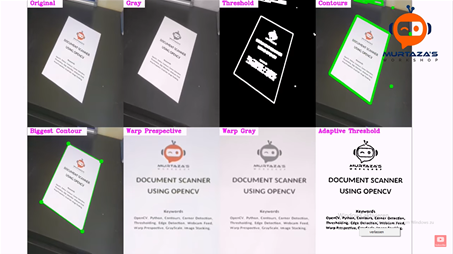
\includegraphics[scale=1]{pics/maperkennung/documentscanner.png}
    \caption{Documenten Scanner}
    \label{fig:map:documentscanner}
\end{figure}

Aus diesen Konturen, welche OpenCV2 erkennt, wird die größte, geschlossene Umrandung herausgesucht. Es wird davon ausgegangen, dass sich hier das fokussierte Objekt, also das Blatt Papier, befindet. Um nun die vier Eckpunkte lokalisieren zu können, wird eine vorgefertigte Funktion namens ``approxPolyDP'' angewendet. Diese legt, mit den übergebenen Parametern ein Viereck über die Konturen. Danach werden aus diesem Viereck die 4 Eckpunkte extrahiert und als Array wieder an den Client zurückgesendet.


\begin{lstlisting}[caption=approxPolyDP,language=Python,label=lst:impl:findBiggestContour]
    def biggestContour(contours, accuracy, areaVal):  # FIND THE BIGGEST CONTOUR
        biggest = np.array([])
        max_area = 0

        for i in contours:
            area = cv2.contourArea(i)
            if area > areaVal:
                peri = cv2.arcLength(i, True)
                # findet die vier Eckpunkte heraus und gibt diese zurueck
                approx = cv2.approxPolyDP(i, accuracy * peri, True)
                if area > max_area and len(approx) == 4:  # IF == 4 THEN SQUARE
                    biggest = approx
                    max_area = area
        return biggest, max_area
\end{lstlisting}

In der folgenden Funktion namens ``getWrappedImg(\dots)'', wird das Bild, welches aufgenommen wurde in eine zwei-dimensionale top-down Ansicht umgewandelt. Allerdings geschieht dies nur da, wo zuerst die Eckpunkte beziehungsweise das Blatt Papier (also die Spielumgebung) gefunden wurden. Wie dies funktioniert ist im folgenden Codeblock
\ref{lst:impl:convertPoints} ersichtlich.


Zuerst wird aus dem übergebenen ``snipset''-Parameter, welcher als Array vorliegt, die Daten ausgelesen und auf die Variablen ``pt\_A'' bis ``pt\_D'' geschrieben. Diese vier Buchstaben geben die Eckpunkte an. Aus diesen Eckpunkten wird im Folgenden dann ein Vektor erzeugt. Für weitere Berechnungen wird dann noch die länge zwischen den wahrscheinlich parallel zueinanderliegenden Vektoren AD und BC berechnet. Dies ist wichtig, um im späteren Code herauszufinden, in welcher Orientierung das Blatt Papier zu der Kamera liegt.

\begin{lstlisting}[caption=Bild in Vogelperspektive umwandeln,language=Python,label=lst:impl:convertPoints]
def getWrappedImg(img, snipset):
    snipset = squarify(snipset)

    pt_A = snipset[0]
    pt_B = snipset[1]
    pt_C = snipset[2]
    pt_D = snipset[3]

    lineAB = np.array([pt_A, pt_B])
    lineBC = np.array([pt_B, pt_C])
    lineCD = np.array([pt_C, pt_D])
    lineDA = np.array([pt_D, pt_A])

    width_AD = np.sqrt(((pt_A[0] - pt_D[0]) ** 2) + ((pt_A[1] - pt_D[1]) ** 2))
    width_BC = np.sqrt(((pt_B[0] - pt_C[0]) ** 2) + ((pt_B[1] - pt_C[1]) ** 2))
\end{lstlisting}
Im folgenden Code-Block passiert zuerst im Grunde genommen genau dasselbe, wie im zuvor erklärtem Code-Block \ref{lst:impl:convertPoints}. Hier wird die größere Länge der beiden Vektoren AB und CD, welche wahrscheinlich in der Realität parallel zueinander liegen, errechnet. Dabei wird angenommen, dass diese beiden Längen die Höhe des Blatt Papiers sind.
\begin{lstlisting}[language=Python,label=lst:impl:findBiggestLine,firstnumber=16]
    maxHeight = max(int(width_AD), int(width_BC))
    if maxHeight == width_AD:
        lineA = lineDA
    else:
        lineA = lineBC

    height_AB = np.sqrt(((pt_A[0] - pt_B[0]) ** 2) +
                        ((pt_A[1] - pt_B[1]) ** 2))
    height_CD = np.sqrt(((pt_C[0] - pt_D[0]) ** 2) +
                        ((pt_C[1] - pt_D[1]) ** 2))
    maxWidth = max(int(height_AB), int(height_CD))
    if maxWidth == height_AB:
        lineB = lineAB
    else:
        lineB = lineCD
\end{lstlisting}

Die nun errechnete maximale Höhe wird nun noch mit einem realistischen Faktor multipliziert, um noch ein akkurateres Ergebnis der Perspektiventransformation erzielen zu können. Dieser ``realistische Faktor'' wird errechnet, indem der Winkel zwischen den beiden größten orthogonal zueinander liegenden Linien in folgende Formel miteinbezogen wird:
\[ factor
    = \dfrac{90}{(180-angle)}
\]
Dieser errechnete Faktor staucht die Höhe eines Bildes, welches von der unteren Blattkante aufgenommen wurde und streckt die Höhe von jene, welche, wieso auch immer, von oben Blattkante aufgenommen wurden.


\begin{lstlisting}[language=Python,label=lst:impl:angle,firstnumber=31]
    angle = ang(lineA, lineB)
    if angle == 90:
        factor = 1
    if angle > 90:
        factor = 90 / (180-angle)
    if angle < 90:
        factor = 90 / angle

    maxHeight *= factor
\end{lstlisting}

Im letzten Teil der Funktion wird lediglich nur noch das Bild in die richtige Perspektive transformiert. Dies wird erzielt, indem man die beiden vorgefertigten Funktionen ``cv2.getPerspectiveTransform(\dots)'' und ``cv2.warpPerspective(\dots)'' verwendet. Als Return-Wert liefert die genannte Funktion ein Bild mit dem Datentypen OpenCV2, welches dann im späteren Verlauf noch umcodiert werden muss.

\begin{lstlisting}[language=Python,label=lst:impl:wrapPerspective,firstnumber=40]
    m = np.array([pt_A, pt_B, pt_C, pt_D])
    m = rotateCW(m)
    input_pts = np.float32(m)
    output_pts = np.float32([[0, 0],
                            [0, maxHeight - 1],
                            [maxWidth - 1, maxHeight - 1],
                            [maxWidth - 1, 0]])

    M = cv2.getPerspectiveTransform(input_pts, output_pts)

    dst = cv2.warpPerspective(
        img, M, (int(maxWidth), int(maxHeight)), flags=cv2.INTER_LINEAR)

    return dst
\end{lstlisting}


\subsection{Open-CV2 [H]}
\subsubsection{Bildverarbeitungsalgorithmen} \label{maai:alogs}

Bildverarbeitungsalgorithmen sind Grundbausteine für die Bild- beziehungsweise Map-Erkennung. Ohne diesen können keine, oder nur wenige Daten aus Bildern ausgelesen werden. Somit würde jedes Bild nur Informationen über die Helligkeit und die Farbe/Farbhelligkeit jedes Bildpunktes beinhalten. Deshalb ist es wichtig Bildverarbeitungsalgorithmen zu verwenden um mehr Informationen aus den Bildern, welche dem Python-Server zur Verfügung gestellt werden, zu erkennen und zu erhalten. In dieser Arbeit wurden folgende Methoden von OpenCV2 verwendet, welche das Erkennen des Blatt Papiers ermöglichten. Im Folgenden (\ref{maai:grayscale}-\ref{maai:wrapPerspective}) wird näher auf die Funktionsweise der einzelnen Algorithmen eingegangen. Diese sind:

\begin{compactitem}
    \item cv2.cvtColor(image, cv2.COLOR\_BGR2GRAY) (``Grayscaling''): Diese Funktion bewirkt eine Graustufenkonvertierung eines gegebenen Bilds.
    \item cv2.GaussianBlur(\dots) (``Blurring''): Mit dieser Funktion wird ein gegebenes Bild unscharf gezeichnet und somit unnötig genaue Informationen entfernt.
    \item cv2.adaptiveThreshold(\dots) (``Adaptive Thresholding''): Hier wird die Schwellwertbildung adaptiv festgelegt. Es wird das gegeben Bild in Raster unterteilt und für jeden dieser Raster ein Schwellwert gebildet. Somit werden Farbübergänge eliminiert und es bleibt ein reines Schwarz-Weiß-Bild mit harten Kanten über.
    \item cv2.canny(\dots) (``Canny'' Kantenerkennung): Die Kantenerkennung liefert automatisch erkannte Kanten aus einem gegebenen Bild.
    \item cv2.approxPolyDP(\dots) (``ApproxPolyDP''): Diese Funktion vergröbert die erkannten Konturen um einen angegebenen Grad. Die erkannten Konturen werden auf wenige Punkte minimiert. Somit kann zum Beispiel über eine Kontur ein Vieleck gelegt werden.
    \item cv2.warpPerspective(\dots) (Perspektiven-Korrektur): Mit ``wrapPerspective'' kann ein Bild, welches in einer weiteren Dimension aufgenommen wurde und somit einer Perspektive unterlag Perspektiven-korrigiert werden.
\end{compactitem}

Nur einige der verwendeten Bildbearbeitungsalgorithmen sind basierend auf Pixelmanipulation. Andere Algorithmen, wie zum Beispiel ``ApproxPolyDP'', sind reines Auslesen von Bildwerten beziehungsweise -daten, welche durch Vorarbeit extrahiert wurden.


\subsubsection{Grayscale}\label{maai:grayscale}
Beim ``grayscaling'' werden Informationen über die Lichtintensität aus den einzelnen Pixeln extrahiert und über eine Gewichtung der drei Farben Rot, Grün und Blau gleichmäßig gewertet. Somit entsteht ein Bild, welches rein Informationen über die Helligkeit/Lichtintensität enthält.

Die Lichtintensität ist die Menge an Licht(stärke) pro Pixel. Diese Lichtstärke kann in einem 8-Bit System von den Farben Rot, Grün und Blau von 0-255 reichen. Der Kontrast geht somit von ganz schwarz, was einer Lichtintensität von 0 entspricht (es wird aus diesem Pixel kein Licht emittiert), bis ganz weiß, was in einem 8-Bit System 255 entspricht.

Für eine Umwandlung eines Bilds in dessen Graustufen wird für jeden Pixel also die Lichtintensität der drei Farben (Rot, Grün und Blau) beziehungsweise der Farbkombination dieser drei Farben gemessen und über eine Gewichtung der drei Werte ein ``Mittelwert'' errechnet. Diese Gewichtung kann über verschiedene Faktoren erfolgen. Daher ist es nicht gegeben, dass auch OpenCV2 die folgende Formel zur Umrechnung eines Bildes, welches aus einem RGB(A)-Farbraum (Rot (R); Grün (G); Blau (B); Opazität (A)) in Graustufen konvertiert werden soll, verwendet. Die Formel dient deswegen nur als Exempel, um alle drei Werte auf eine lineare Gleichgültigkeit für das menschliche Auge zu setzen, um somit ein Graustufenbild zu erzeugen:

\[
    Y_{ linear } = 0,2126 * R_{ linear } + 0.7152 * G_{ linear } + 0.0722 * B_{ linear }
\]

Aus dieser Formel ist erkennbar, dass die Farbe Grün mehr gewichtet wird als Rot und Blau. Dies resultiert daraus, dass das Auge die meiste Lichtinformation aus der Farbe Grün extrahieren kann. Somit wirkt auch diese Farbe am hellsten für das menschliche Auge. Deshalb wird sie am höchsten gewichtet, damit ein scheinbar ausgeglichener Wert der Lichtintensität der Farbkombination der drei Farben herauskommt. Dieser gewichtete Wert (Y), welcher auch als Luminanz bezeichnet wird, ist die Basis für die Graustufenkonvertierung.

Im folgendem Code-Beispiel \ref{maai:grayscaling} wird die Umsetzung einer Graustufenkonvertierung mittels OpenCV2 in der Programmiersprache Python gezeigt.
% Quelle: https://en.wikipedia.org/wiki/Grayscale

\begin{lstlisting}[caption=Graustufenkonvertierung,language=Python,label=maai:grayscaling]
    # OpenCV2 used as pixel manipulation library
    import cv2
  
    # read Image from Folder
    image = cv2.imread('Path/to/your/image.jpg')
    # Convert RGB image to (2) gray
    gray = cv2.cvtColor(image, cv2.COLOR_BGR2GRAY)
    
    # display the original image (input) on the screen
    cv2.imshow('Original image',image)
    # display the grayscaled image (output of cv2 funktion cvtColor) on the screen
    cv2.imshow('Gray image', gray)
      
    cv2.waitKey(0) # waits until a key is pressed
    cv2.destroyAllWindows() # destroys the window showing image
\end{lstlisting}
%Quelle: Zitat: https://docs.opencv.org/3.4/d8/d01/group__imgproc__color__conversions.html

Dieses Stück Programmcode führt zu folgendem Ergebnis:

\begin{figure}[htb]
    \centering
    \begin{minipage}[t]{0.45\linewidth}
        \centering
        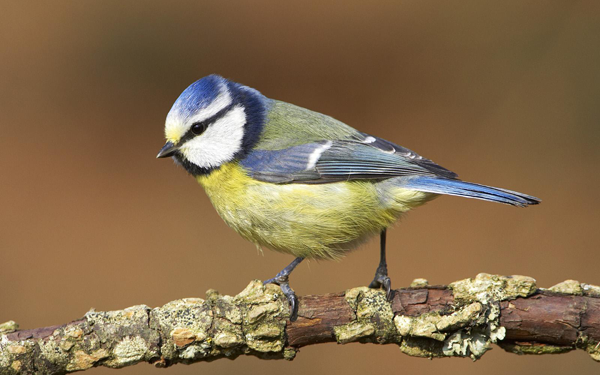
\includegraphics[width=\linewidth]{pics/bildverarbeitungsalgos/input.png}
        \caption{Input}
        \label{maai:grayscaling:input}
    \end{minipage}
    \hfill
    \begin{minipage}[t]{0.45\linewidth}
        \centering
        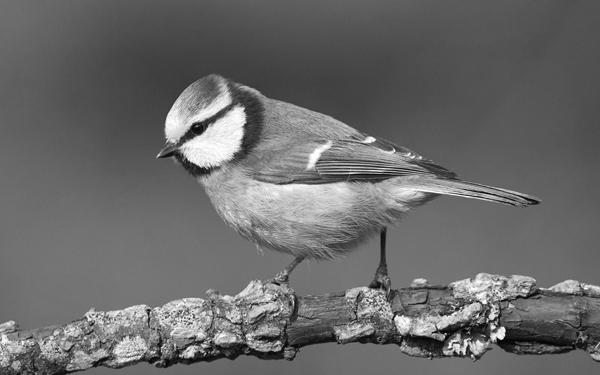
\includegraphics[width=\linewidth]{pics/bildverarbeitungsalgos/grayscaling_output.png}
        \caption{Output}
        \label{maai:grayscaling:output}
    \end{minipage}
\end{figure}
%Quelle: https://s3.envato.com/files/16109405/index.html

\subsubsection{Blurring}\label{maai:blurring}

Soll ein Bild ``geblurred'' (engl. für verwischen/verschwommen) werden, so ist das Ziel eine Unschärfe. Ähnlich, wie das ``Grayscaling'' ist auch das unscharf-Zeichnen eines Bildes reine Pixelmanipulation. Hier wird jedoch nicht ein einzelner Pixel zur Berechnung der Unschärfe herangezogen, sondern eine zweidimensionale Matrix an umliegenden Bildpunkten. Somit wird jeder Pixel basierend auf dessen benachbarten Bildzellen manipuliert.

Um eine Unschärfe zu erzielen, muss eine mathematische Operation der Faltung einer spezialisierten Matrix, genannt Kernel, auf die Matrix des Bildes angewandt werden. Dabei wird diese Faltungsoperation auch ``Konvolution'' genannt.

Mathematisch gesehen ist Konvolution, also die Faltung zweier Matrizen, A mit der Größe a \(\times\) b und B mit der Größe c \(\times\) d, eine \((a + c -1) \times (b + d - 1)\) Matrix C mit folgenden Einträgen:
\[
    C_{ rs } = \sum_{i+k=r+1, j+l=s+1}^{r=a+c-1,s = b + d - 1} A_{ ij }B_{ kl }
\]
Aus dieser Formel ist ersichtlich, dass das Falten beziehungsweise die Konvolution zweier Matrizen A und B eine neue Matrix C, in welcher die Einträgen durch die Summe des Produkts der Einträge der Matrix A mit den am gleich liegenden zweidimensionalen Indexe entsprechenden Einträgen der anderen Matrix B gebildet werden, erzeugt. Alle diese Produkte werden im zweidimensionalen, also entlang den Zeilen und Spalten, berechnet.

Der zuvor genannte (Begriff) Kernel kann als Matrix beschrieben werden. Diese dient dazu ein Bild in dessen Aussehen zu verändern. Somit ist der Begriff nicht nur auf das Weichzeichnen von Bildern begrenzt. Ein Kernel kann zum Beispiel auch dazu verwendet werden, um Kanten in Bildern zu schärfen.

Da der Kernel eine Matrix mit einem Mittelpunkt ist, muss die Kernel Größe einer ungeraden Zahl, zum Beispiel \([5*5]\), entsprechen.

In dieser Diplomarbeit wurde häufig der ``Gauß'scher'' Weichzeichnungsfilter verwendet. Dieser Filter gibt jedem Bildpunkt, welche um einen betrachteten Pixel liegen, eine Gewichtung.

Diese Gewichtung nimmt mit der Distanz zu dem betrachteten Pixel ab. Somit hat theoretisch jeder Pixel in der Bild-Matrix eine eigene Gewichtung. Da diese jedoch mit der Distanz so stark abnehmen werden diese nicht mehr berücksichtigt. Die theoretische Formel zur Berechnung der Gewichte der Pixelwerte rund um einen fokussierten Bildpunkt sieht wie folgt aus:
\[
    G(x,y)=\frac{ 1 }{ 2*\pi*\sigma^2 }*e^{ - \frac{ x^2 + y^2 }{ 2*\sigma^2 } }
\]
Wobei x und y der horizontale und vertikale Abstand zum untersuchten Bildpunkt ist. Sigma ist die Standardabweichung (je höher der Wert von Sigma, desto stärker ist auch der Weichzeichnungseffekt).

In der Realität werden jedoch die Werte dieser ``Gaus'schen'' Funktion mittels der Werte im Kernel genähert. Dabei macht es wenig Sinn, dass die Kernel-Matrix groß gewählt wird, da der Wert eines Eintrags im Kernel mit der Distanz zum Mittelpunkt abnimmt. Dabei wird oft das \(\sigma\) der Funktion in der Programmierung ignoriert und vom Programm auf Basis der angegebenen Größe des Kernels selbst entschieden. Somit sieht eine Näherung an die ``Gaus'sche'' Formel durch eine Kernel Matrix wie folgt aus:
\[
    \frac{ 1 }{ 16 } * \left[\begin{array}{rrr}
            1 & 2 & 1 \\
            2 & 4 & 2 \\
            1 & 2 & 1 \\
        \end{array}\right]
\]
OpenCV2 stellt jedoch bereits Funktionen zur Verfügung, welche das Kalkulieren des Kernels abnimmt. Im folgendem Codeblock (\ref{maai:gaussianblur}) wird gezeigt, wie diese Funktion in dieser Arbeit verwendet wurde.

% Quelle: https://medium.com/swlh/how-image-blurring-works-652051aee2d1

\begin{lstlisting}[caption=Gaussian Blur,language=Python,label=maai:gaussianblur]
    import cv2
    import numpy
    
    # read image
    src = cv2.imread('/path/to/image.png', cv2.IMREAD_UNCHANGED)
    
    # apply guassian blur on src image
    # (10,10) is the Kernel size
    dst = cv2.GaussianBlur(src,(10,10),cv2.BORDER_DEFAULT)
    
    # display input and output image
    cv2.imshow("Gaussian Smoothing",numpy.hstack((src, dst)))
    cv2.waitKey(0) # waits until a key is pressed
    cv2.destroyAllWindows() # destroys the window showing image
\end{lstlisting}

%Quelle: https://www.tutorialkart.com/opencv/python/opencv-python-gaussian-image-smoothing/

Führt man diesen Programmcode aus, so erzeugt dieser folgenden Effekt:

\begin{figure}[htb]
    \centering
    \begin{minipage}[t]{0.45\linewidth}
        \centering
        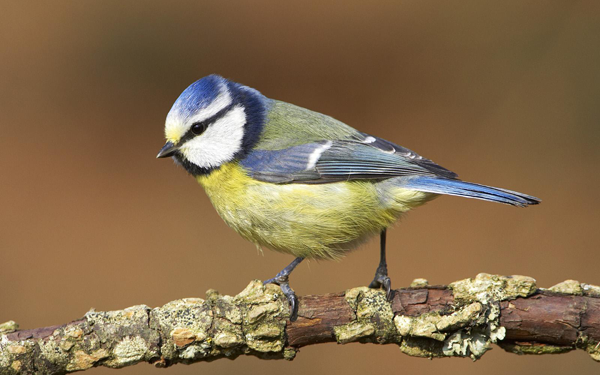
\includegraphics[width=\linewidth]{pics/bildverarbeitungsalgos/input.png}
        \caption{Input}
        \label{maai:gaussianblur:input}
    \end{minipage}
    \hfill
    \begin{minipage}[t]{0.45\linewidth}
        \centering
        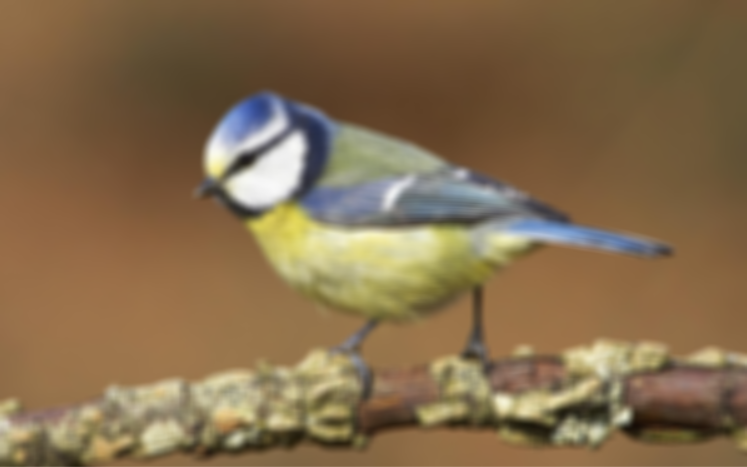
\includegraphics[width=\linewidth]{pics/bildverarbeitungsalgos/gaussianblur_output.png}
        \caption{Output}
        \label{maai:gaussianblur:output}
    \end{minipage}
\end{figure}

% Quelle: https://www.tutorialkart.com/opencv/python/opencv-python-gaussian-image-smoothing/

\subsubsection{Thresholding}

Das ``Image-Thresholding'' also die Schwellwertbildung eines Bilds ist basierend auf die ``Image-Segmentation''. Diese erzeugt eine Unterteilung eines Bildes in mehrere Segmente.

Das ``Image-Thresholding'' ist eine einfache Form der Segmentierung. Das ``Thresholding'' basiert auf gesetzte Schwellwerte, welches unterschiedlich ``intensive'' Pixel trennen soll. Dadurch ist das Produkt ein binäres Bild, welches aus Nullen und Einsen besteht (= entweder hell oder dunkel).

``Thresholding'' ist, wie auch die Graustufenkonvertierung (Kapitel ``Grayscaling'' \ref{maai:grayscale}), das Weichzeichnen von Bildern (Kapitel ``Blurring'' \ref{maai:blurring}) und viele andere Methoden der Bildverarbeitung, eine Art der Pixelmanipulation. Die Pixel sollen beim ``Image-Thresholding'' beziehungsweise bei der Schwellwertbildung so angepasst werden, dass Bilder und deren Pixel einfacher zu analysieren sind. In dieser Arbeit legte das Schwellwert-Bild den Grundbaustein zur Konturen-/Kantenerkennung.

Ziel ist es also, aus einem Farb- beziehungsweise Graustufenbild eine Segmentierung zu erzeugen. Durch dieses Verfahren wird also, wie zuvor erwähnt, ein binäres Bild erzeugt, welches nur noch Schwarz- und Weißwerte beinhaltet. Dies wird zum Beispiel dafür verwendet, dass ein Hintergrund vom Vordergrund getrennt wird. Somit werden sogenannte ``Regions Of Interest'' erkannt. ``Region Of Interest'' bedeutet ``Bereich von Interesse''. Hierzu werden spezielle Bereiche aus einem Histogramm, also einer Messkurve, ausgewertet beziehungsweise ausgewählt und nach dem zuvor definierten Schwellwert in Gruppen unterteilt. Somit gibt die ``Region Of Interest'' die fokussierten/für die Auswertung Interessanten Bereiche eines Bildes wieder. Dem Hintergrund wird in einem binären Bild der Wert 0 (null) zugewiesen und dem Vordergrund der Wert 1. Diese Werte werden in einem Bild als 0 (null) - schwarz und als 1 – Weiß dargestellt.

Durch das ``Thresholding'' gibt es die Möglichkeit ein Histogramm zu erstellen, um die Helligkeitswerte eines Bildes zu analysieren. Wenn man aus diesem Graustufenbild (\ref{maai:thresholding:input}) ein Histogramm (\ref{maai:thresholding:histogramm}) erzeugt, sieht dies wie folgt aus:

\begin{figure}[htb]
    \centering
    \begin{minipage}[t]{0.45\linewidth}
        \centering
        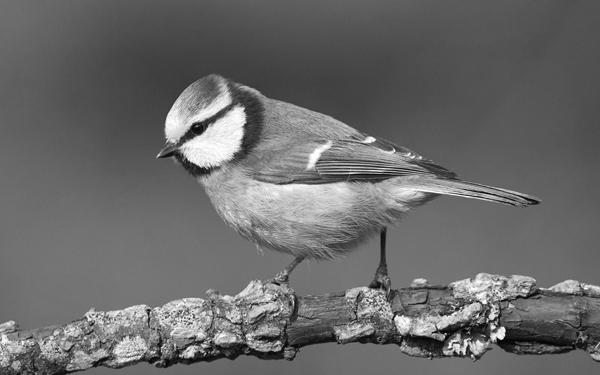
\includegraphics[width=\linewidth]{pics/bildverarbeitungsalgos/grayscaling_output.png}
        \caption{Input}
        \label{maai:thresholding:input}
    \end{minipage}
    \hfill
    \begin{minipage}[t]{0.45\linewidth}
        \centering
        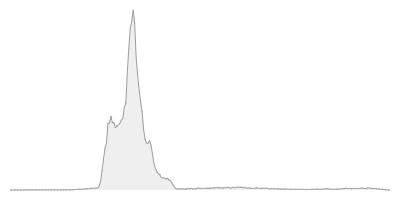
\includegraphics[width=\linewidth]{pics/bildverarbeitungsalgos/thresholding_histogram.png}
        \caption{Helligkeitsverteilung}
        \label{maai:thresholding:histogramm}
    \end{minipage}
\end{figure}

Das Histogramm veranschaulicht die Helligkeitsverteilung aller Pixel von den Werten 0 (null) (schwarz), welcher der Wert ganz Links auf der X-Achse im Histogramm ist, bis 255 (weiß), welches dem äußersten X-Wert entspricht. Auf der Y-Achse befindet sich die Häufigkeit der vorkommenden Pixel mit der entsprechenden Helligkeit.
Man kann also erkennen und analysieren, dass überwiegend Hintergrund (dunkle Helligkeitswerte) in diesem Bild existiert. Damit aus diesem Histogramm auch ein Schwellwert-Bild (das binäre Bild) erzeugt werden kann, wird ein zuvor definierter Schwellwert zur Verarbeitung der Pixel herangezogen. Somit werden global (!) nur alle Pixel über einem gewissen Helligkeitswert in den Wert 1 (Vordergrund) umgewandelt. Alle anderen bleiben Schwarz. Sieht man sich nun folgendes Bild (\ref{maai:thresholding:output}) an, kann man durch die Schwellwertbildung erkennen, dass sich das interessante Objekt in der Bildmitte befindet:


\begin{figure}[htb]
    \centering
    \begin{minipage}[t]{0.45\linewidth}
        \centering
        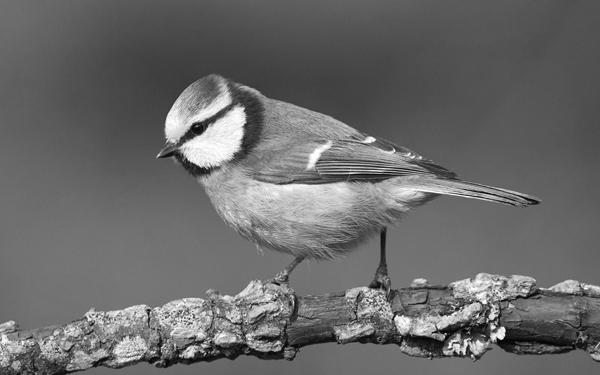
\includegraphics[width=\linewidth]{pics/bildverarbeitungsalgos/grayscaling_output.png}
        \caption{Input}
        \label{maai:thresholding:input:second}
    \end{minipage}
    \hfill
    \begin{minipage}[t]{0.45\linewidth}
        \centering
        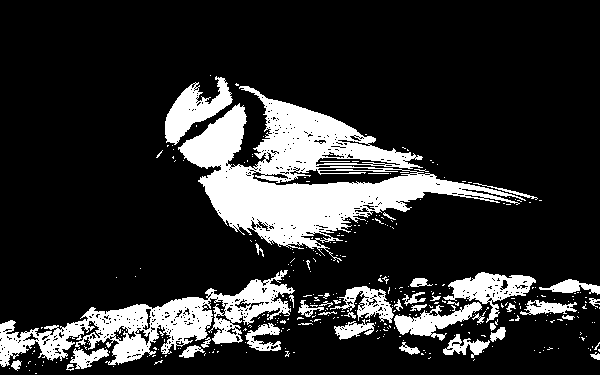
\includegraphics[width=\linewidth]{pics/bildverarbeitungsalgos/thresholding_output.png}
        \caption{Output}
        \label{maai:thresholding:output}
    \end{minipage}
\end{figure}
%Quelle: https://www.youtube.com/watch?v=8TkligJJCAQ&ab_channel=Apeer_micro
%Quelle: https://datacarpentry.org/image-processing/07-thresholding/


Für dieses Bild wurde ein globaler Schwellwert verwendet. Dies ist jedoch keine gute Entscheidung, wenn der Helligkeitseinfall im Bild unterschiedlich stark ist. In unserer Arbeit wurde daher ein adaptiver Schwellwert verwendet. Dieser wird somit durch einen Algorithmus für einen Pixel basierend auf einem kleinen Bereich um ihn herum gebildet. Dadurch werden unterschiedliche Schwellwerte in unterschiedlichen Regionen des Bildes gebildet, um eine ungleichmäßige Beleuchtung zu korrigieren.

%Quelle: https://docs.opencv.org/4.x/d7/d4d/tutorial_py_thresholding.html
Programmiertechnisch wurde dies wie folgt umgesetzt:


\begin{lstlisting}[caption=Adaptive Gaussian Thresholding,language=Python,label=maai:gaussianthresholding]
    # Python program to illustrate
    # adaptive thresholding type on an image
    
    # organizing imports
    import cv2
    import numpy as np
    
    # path to input image is specified and
    # image is loaded with imread command
    image1 = cv2.imread(
        'path/to/img.png')
    
    # cv2.cvtColor is applied over the
    # image input with applied parameters
    # to convert the image in grayscale
    img = cv2.cvtColor(image1, cv2.COLOR_BGR2GRAY)
    
    # applying gaussian thresholding
    # technique on the input image
    thresh = cv2.adaptiveThreshold(
        img, 255, cv2.ADAPTIVE_THRESH_GAUSSIAN_C, cv2.THRESH_BINARY_INV, 5, 4)
    
    cv2.imshow('Adaptive Gaussian', thresh)
    
    
    # De-allocate any associated memory usage
    if cv2.waitKey(0) & 0xff == 27:
        cv2.destroyAllWindows()
\end{lstlisting}
%Quelle: https://www.geeksforgeeks.org/python-thresholding-techniques-using-opencv-set-2-adaptive-thresholding/

Dieser Code erzeugt aus einem Input-Bild (\ref{maai:thresholding:input:thrid}) folgendes Schwellwert-Bild (\ref{maai:gaussianthresholding:output}), in welchem sehr genau erkennbar ist, was den Vordergrund bildet.


\begin{figure}[htb]
    \centering
    \begin{minipage}[t]{0.45\linewidth}
        \centering
        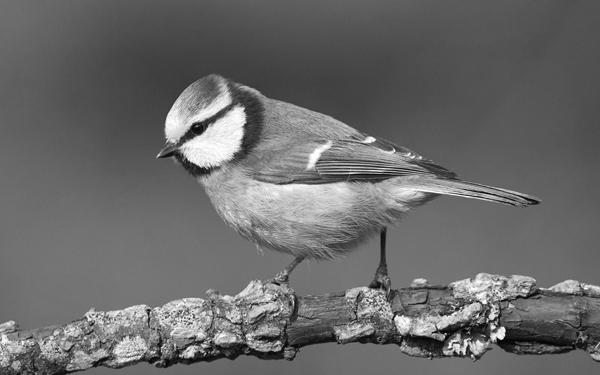
\includegraphics[width=\linewidth]{pics/bildverarbeitungsalgos/grayscaling_output.png}
        \caption{Input}
        \label{maai:thresholding:input:thrid}
    \end{minipage}
    \hfill
    \begin{minipage}[t]{0.45\linewidth}
        \centering
        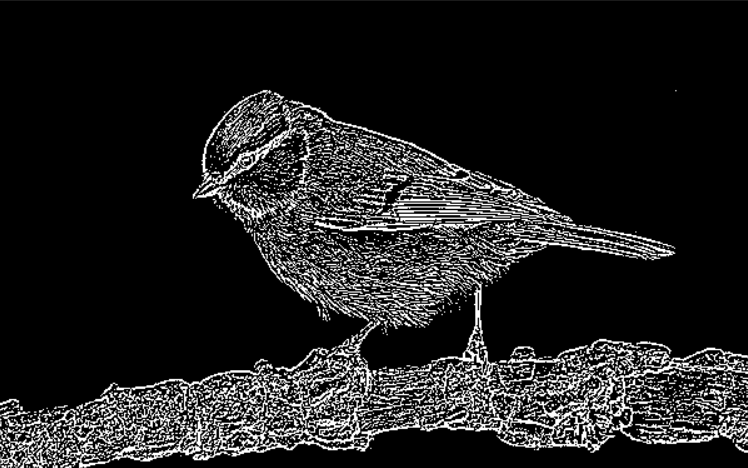
\includegraphics[width=\linewidth]{pics/bildverarbeitungsalgos/gaussian_thresholding.png}
        \caption{Output}
        \label{maai:gaussianthresholding:output}
    \end{minipage}
\end{figure}

\subsubsection{Detecting Contours}

Kantenerkennung ist wie die Graustufenkonvertierung (\ref{maai:grayscale}) oder das Weichzeichnen (\ref{maai:blurring}) ein Bildverarbeitungsalgorithmus, welcher dazu verwendet wird, um Diskontinuitäten zu identifizieren. Hierzu werden scharfe Änderungen der Bildfarbe/der Bildintensität herausgefiltert. Punkte, wo dieser Wert stark variiert, wird als Kante abgestempelt.

Das Kanten erkennen schafft eine Basis für die Bildverarbeitung und Form Erkennung der Bild- und Objekterkennung. Für die Konturenerkennung sind jedoch nur geschlossene Kanten von Bedeutung.

Die Kantenerkennung funktioniert wie folgt. Für die ``Edge-Detection'' (Kantenerkennung) ist wie beim Weichzeichnungsalgorithmus (\ref{maai:blurring}) eine Konvolution nötig; vor allem, um hochauflösende Bilder zu verarbeiten. Oft wird dazu der sogenannte ``Sobel''-Operator herangezogen. Dieser erzeugt für die Kantenerkennung zwei Kernel, welche in x- und y-Richtung unterteilt sind. Der Kernel in x-Richtung sieht wie folgt aus:

\[
    \left[\begin{array}{rrr}
            -1 & 0 & 1 \\
            -2 & 0 & 2 \\
            -1 & 0 & 1 \\
        \end{array}\right]
\]


Hier sind negative Nummern links und positive Nummern rechts. Wegen der 0 (null) in der Mitte des Kernels wird nur geprüft, ob eine vertikale Linie/Kontur nach unten existiert. Daher wird mit diesem Kernel nur in x-Richtung auf eine Kante überprüft. Die mittigen Pixel auf der y-Achse des Kernels werden durch den ``Sobel''-Operator höher gewichtet als die Randpixel.

Das Ziel ist dabei einen Unterschied zwischen der Farb-/Lichtintensität des linksseitigen Bereichs des Bilds (der Pixel auf der linken Seite) und der Intensität des rechtsseitigen Bereichs des Bilds (der Pixel auf der rechten Seite) herauszufinden.

Anhand eines Beispiels wird diese Operation klarer:

\[
    \left[\begin{array}{rrrr}
            0 & 0 & 255 & 255 \\
            0 & 0 & 255 & 255 \\
            0 & 0 & 255 & 255 \\
            0 & 0 & 255 & 255 \\
        \end{array}\right]
\]

Hier existiert eine für einen Menschen klar erkennbare Kante; jedoch tut sich bei dem Erkennen die Maschine etwas schwerer. Dazu muss der zuvor genannte Kernel über die Pixel gelegt werden. So erhält man durch die Summe der Multiplikationen der einzelnen Werte des Kernels mit den entsprechenden Werten der Matrix des Bildes. Diese ergibt in diesem Beispiel 1025. Ist dieser Wert über einen zuvor definierten Schwellwert, so existiert an dieser Position eine Kante.

Für die Konturenerkennung wird ein Bereich von geschlossenen Kanten herangezogen. Diese geschlossenen Kanten werden erkannt, indem eine Kante in einem zuvor definierten Kernel rund um eine weitere Kante existiert. Führt dieser Pfad wieder zurück zur Ausgangskante, so kann mit Sicherheit gesagt werden, dass es sich um eine Geschlossene Kontur handelt.

%Quelle:https://www.geeksforgeeks.org/find-and-draw-contours-using-opencv-python/


\begin{lstlisting}[caption=Adaptive Gaussian Thresholding,language=Python,label=maai:gaussianthresholding]
    
import cv2
import numpy as np

# Let's load a simple image with 3 black squares
image = cv2.imread(
    'path/to/image.png')
cv2.waitKey(0)

# Grayscale
gray = cv2.cvtColor(image, cv2.COLOR_BGR2GRAY)

# Find Canny edges
edged = cv2.Canny(gray, 30, 200)
cv2.waitKey(0)

# Finding Contours
# Use a copy of the image e.g. edged.copy()
# since findContours alters the image
contours, hierarchy = cv2.cv2.findContours(
    edged, cv2.RETR_LIST, cv2.CHAIN_APPROX_SIMPLE)

cv2.imshow('Canny Edges After Contouring', edged)
cv2.waitKey(0)

print("Number of Contours found = " + str(len(contours)))

# Draw all contours
# -1 signifies drawing all contours
cv2.drawContours(image, contours, -1, (255, 255, 0), 1)

cv2.imshow('Contours', image)
cv2.waitKey(0)
cv2.destroyAllWindows()

\end{lstlisting}

Dieser Programmcode erzeugt folgendes Bild:


\begin{figure}[htb]
    \centering
    \begin{minipage}[t]{0.45\linewidth}
        \centering
        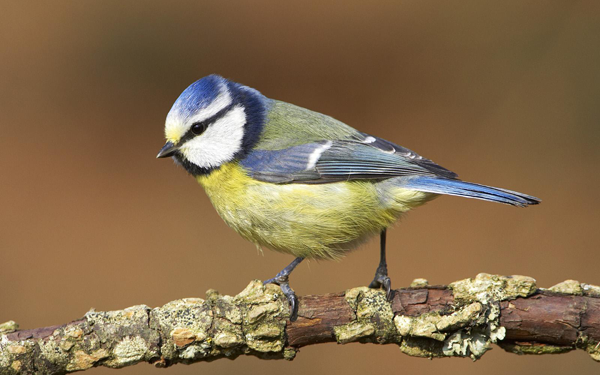
\includegraphics[width=\linewidth]{pics/bildverarbeitungsalgos/input.png}
        \caption{Input}
        \label{maai:getcounturs:input}
    \end{minipage}
    \hfill
    \begin{minipage}[t]{0.45\linewidth}
        \centering
        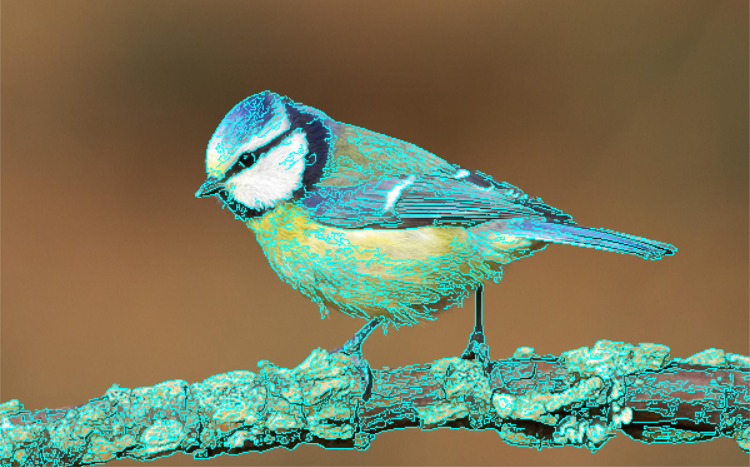
\includegraphics[width=\linewidth]{pics/bildverarbeitungsalgos/getcounturs_output.png}
        \caption{Output}
        \label{maai:getcounturs:output}
    \end{minipage}
\end{figure}

\subsubsection{ApproxPolyDP}\label{maai:approxpolydp:header}

%Quelle: https://pyimagesearch.com/2021/10/06/opencv-contour-approximation/

Um nun aus den gewonnenen Konturen ein Blatt Papier zu erkennen, müssen die vier Eckpunkte des Blattes herausgefunden werden für eine Perspektiventransformation. Diese vier Punkte werden über die Open-Computer-Vision-Funktion ``approxPolyDp(\dots)'' (``approxymation of Polygon Points'' englisch für Annäherung von Polygonen) gewonnen. Die Funktion gibt aus einem übergebenen Konturen-Array (Array = Ansammlung an Daten; in diesem Fall eine Sammlung an Positionsdaten der Kontur-Eckpunkte), eine Annäherung der Eckpunkte zurück. In dem Feld werden die Punkte der Konturen als Vektoren angegeben. Die Annäherung an diese Punkte erfolgt mit einer übergebenen Genauigkeit, welche als Parameter der Funktion spezifiziert wird.

Diese Kontur Näherung, welche den ``Ramer–Douglas–Peucker'' Algorithmus (abgekürzt RDP.; Abbildung \ref{fig:map:rdpalgo}) verwendet, hat das Ziel eine Kontur, also eine Polygon-Line, zu vereinfachen. Dies passiert, indem der Algorithmus die Scheitelpunkte der Kontur bei einem gegebenen Schwellwert reduziert.


\begin{figure}[H]
    \centering
    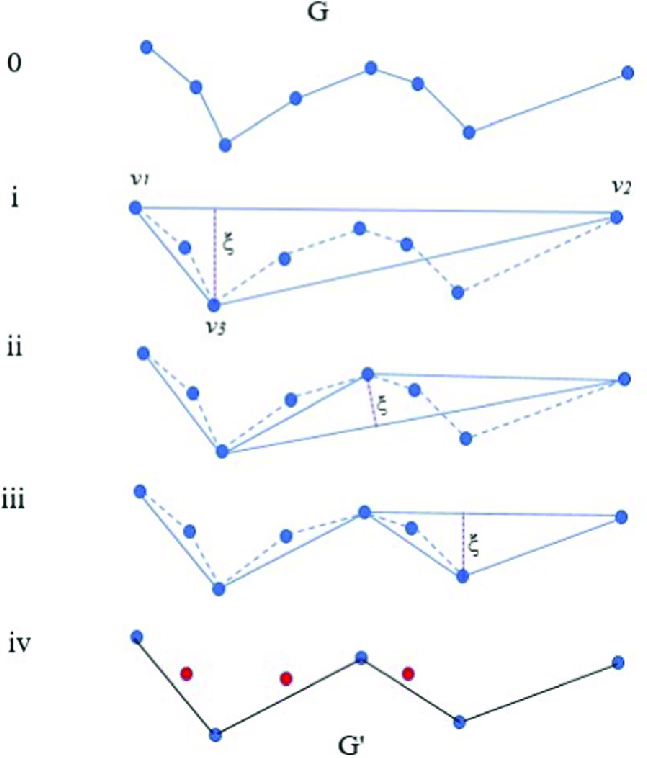
\includegraphics[scale=0.5]{pics/bildverarbeitungsalgos/The-Ramer-Douglas-Peucker-algorithm.png}
    \caption{Der Ramer–Douglas–Peucker Algorithmus}
    \label{fig:map:rdpalgo}
\end{figure}
% Quelle: https://www.researchgate.net/figure/The-Ramer-Douglas-Peucker-algorithm_fig6_332499235

Wenn die Start- und Endpunkte einer Kurve gegeben sind, findet der Algorithmus zuerst den am weitest entfernten Punkt (Endpunkt). Dieser nimmt dann mit einem gegebenen Schwellwert \(x\) einen Bruchteil, welcher zu der Anzahl \(x\) an Polygonpunkten führt, der originalen Kontur her. Der gefragte Punkt, welcher sich an der Stelle des Bruchteils befindet, wird als neuer Konturpunkt herangezogen. Wenn andere Kontur-Punkte dazwischen liegen, so werden diese für den neuen, vereinfachten Konturen-Array ignoriert beziehungsweise eliminiert. Somit werden bestimmte Vertices (Eckpunkte) systematisch eliminiert.

Über bleibt eine Annäherung an eine Ausgangskurve. Somit bleibt am Ende genügend Information über, um zum Beispiel ein Blatt Papier erkennen zu können, was das Hauptziel von diesem Teil der Arbeit (Maperkennung) war. Dabei werden so viel wie möglich Daten aus den Konturen entfernt und die Verarbeitung kann schneller passieren.

Dieses Verfahren wird auch als Kurvenglättung bezeichnet.

Außerdem werden maximal vier Punkte für eine Perspektiventransformation herangezogen.

Das heißt, dass die Scheitelpunkte einer Kurve reduziert werden und dabei trotzdem eine große Menge beziehungsweise Genauigkeit an Information erhalten bleibt. Somit bleibt ein Großteil der Form beibehalten.

Somit werden die vier Eckpunkte des Blatt Papiers in dieser Arbeit herausgefunden. Diese vier Eckpunkte sind eine sehr genaue Annäherung an die Eckpunkte, so wie diese in der Realität vorzufinden sind.

Wie dies mit Python und OpenCV2 umgesetzt wurde, wird im folgenden Codebeispiel ersichtlich:


\begin{lstlisting}[language=Python,caption=ApproxPolyDP Beispiel,label=maai:approxpolydp:code]
    #importing the module cv2
    import cv2

    #reading the image whose shape is to be detected using imread() function
    imageread = cv2.imread('Path/to/image.png')

    #converting the input image to grayscale image using cvtColor() function
    imagegray = cv2.cvtColor(imageread, cv2.COLOR_BGR2GRAY)

    #using threshold() function to convert the grayscale image to binary image
    _, imagethreshold = cv2.threshold(imagegray, 245, 255, cv2.THRESH_BINARY_INV)

    #finding the contours in the given image using findContours() function
    imagecontours, _ = cv2.findContours(imagethreshold, cv2.RETR_TREE, cv2.CHAIN_APPROX_SIMPLE)

    #for each of the contours detected, the shape of the contours is approximated using approxPolyDP() function and the contours are drawn in the image using drawContours() function
    for count in imagecontours:
    epsilon = 0.01 * cv2.arcLength(count, True)
    approximations = cv2.approxPolyDP(count, epsilon, True)
    cv2.drawContours(imageread, [approximations], 0, (0), 3)
    
    #displaying the resulting image as the output on the screen
    cv2.imshow("Resulting_image", imageread)
    cv2.waitKey(0)
\end{lstlisting}
%Quelle: Zitat: https://www.educba.com/opencv-approxpolydp/

Dieser Programmcode führt zu folgendem Ergebnis:


\begin{figure}[htb]
    \centering
    \begin{minipage}[t]{0.45\linewidth}
        \centering
        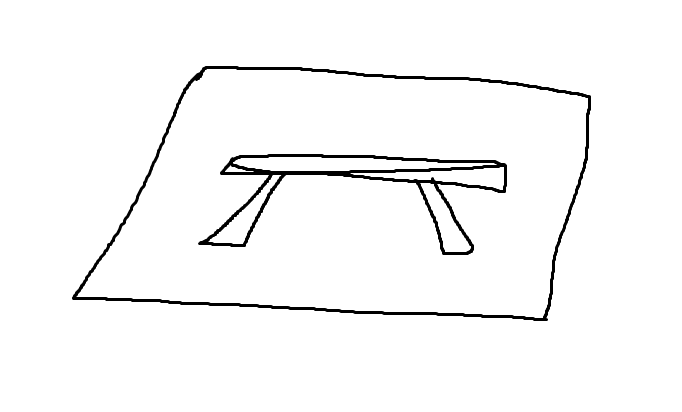
\includegraphics[width=\linewidth]{pics/bildverarbeitungsalgos/ApproxPolyDP_input.png}
        \caption{Input}
        \label{maai:approxpolydp:input}
    \end{minipage}
    \hfill
    \begin{minipage}[t]{0.45\linewidth}
        \centering
        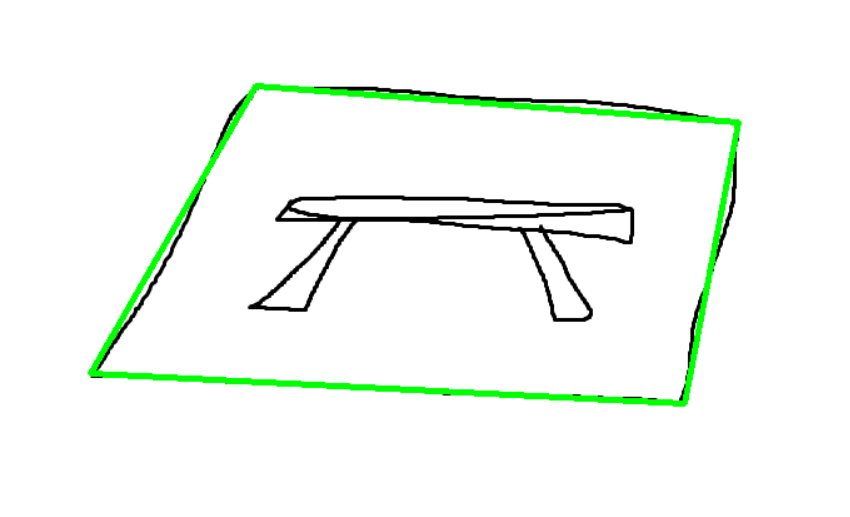
\includegraphics[width=\linewidth]{pics/bildverarbeitungsalgos/ApproxPolyDP_output.png}
        \caption{Erster Output des Programmcodes}
        \label{maai:approxpolydp:output}
    \end{minipage}
\end{figure}


\subsubsection{Wrap Perspective}\label{maai:wrapPerspective}

``Warp Perspective'' ist Englisch und bedeutet ``Perspektiventransformation''. Der Bildverarbeitungsalgorithmus wird zur Perspektivenveränderung herangezogen. Dieser Algorithmus ist der letzte Schritt der Bildverarbeitung, welcher nötig ist, um das Blatt Papier, auf welchem eine Map gezeichnet ist, aus einem Bild zu erkennen.

Durch die Perspektiventransformation werden Winkel, Parallelität und Längen verändert, wodurch es zu einer Stauchung beziehungsweise Streckung eines Bildes kommt.

Der Algorithmus zur Transformation der Perspektive kann wie folgt beschrieben werden:
\[
    \left[\begin{array}{r}
            ti\_x' \\
            ti\_y' \\
            ti     \\
        \end{array}\right]
    = \left[\begin{array}{rrr}
            a_{ 1 } & a_{ 2 } & b_{ 1 } \\
            a_{ 3 } & a_{ 4 } & b_{ 2 } \\
            c_{ 1 } & c_{ 2 } & 1       \\
        \end{array}\right]
    * \left[\begin{array}{r}
            x \\
            y \\
            1 \\
        \end{array}\right]
\]
Auf der rechten Seite der Gleichung befindet sich die Transformationsmatrix als erster Faktor und der Input \(x\) und \(y\) als Vektor und 1 als zweiter Faktor.

Das Produkt daraus, also die linke Seite der Gleichung, gibt den Skalierungsfaktor an. Das heißt der Perspektiven-transformierte Punkte mit den Koordinaten \(x\) und \(y\) wird zu einem neuen Punkt \(P'\) mit den Koordinaten \(x'\) und \(y'\).

Die Transformationsmatrix ist eine Kombination aus folgenden Werten:
\[
    \left[\begin{array}{rr}
            a_{ 1 } & a_{ 2 } \\
            a_{ 3 } & a_{ 4 } \\
        \end{array}
        \right]
    \to
    \text{ Transformation hinsichtlich Rotation, Skalierung, etc. }
\]
\[
    \left[\begin{array}{r}
            b_{ 1 } \\
            b_{ 2 } \\
        \end{array}
        \right]
    \to
    \text{ Verschiebungsvektor }
\]
\[
    \left[\begin{array}{rr}
            c_{ 1 } & c_{ 2 } \\
        \end{array}
        \right]
    \to
    \text{ Projektionsvektor }
\]

Die acht Unbekannten in der Transformationsmatrix geben die Freiheitsgrade im Raum an.

Um die Matrix kalkulieren zu können müssen zuerst die vier Punkte der Eckpunktnäherung durch ``approxPolyDp'' herangezogen werden. Diese Funktion wurde im Kapitel \ref{maai:approxpolydp:header} erklärt. Die vier Eckpunkte, welche in die Vogelperspektive transformiert wurden, sollen ein neues Rechteck darstellen. Das heißt, dass die vier Punkte, welche zuvor im dreidimensionalen Raum die vier Ecken des Blatt Papiers darstellten, werden nun in ein Rechteck perspektiventransformiert. Dadurch wird das Bild in eine Perspektive, welche einen Blick von ``oben'' ermöglicht, umgewandelt, und richtig sakliert.

Somit hat man acht Unbekannte und acht Gleichungen wodurch die Gleichungen in der Matrix-Form gelöst werden können. In OpenCV2 passiert diese Matrixkalkulation via der Funktion ``cv2. getPerspectiveTransform(points, points')''. Der erste Parameter stellt die Koordinaten im Ausgangsbild dar und der zweite stellt die Koordinaten im Ausgabebild dar.

Danach wird ``cv2.wrapPerspective(\dots)'' angewendet, um die Perspektive anhand der gegebenen Matrix zu verändern. Dafür wird aus dem Ausgangsbild ein Teil weggeschnitten und über bleibt der für das ``use-case'' (Anwendungsfall) interessante Teil. Es wird nur jenes Stück aus dem Bild verwendet, welches in den vier gewählten Eckpunkten liegt. Dieses wird in die Vogelperspektive umgewandelt.

Folgender Programmcode zeigt die Matrixrechnung anhand der Bibliothek OpenCV2 und der dazugehörigen Funktionen:



\begin{lstlisting}[language=Python,caption=Perspektiventransformation Beispiel,label=maai:approxpolydp:code]
    #importing the module cv2 and numpy
    import cv2
    import numpy as np

    #reading the image whose perspective is to be changed
    imageread = cv2.imread('C:/Users/admin/Desktop/plane.jpg')
    
    #specifying the points in the source image which is to be transformed to the corresponding points in the destination image
    points1 = np.float32([[0, 100], [700, 260], [0, 700], [700, 400]])
    points2 = np.float32([[0, 200], [600, 0], [0, 700], [1000, 700]])
    
    #applying getPerspectiveTransform() function to transform the perspective of the given source image to the corresponding points in the destination image
    resultimage = cv2.getPerspectiveTransform(points1, points2)
    
    #applying warpPerspective() function to fit the size of the resulting image from getPerspectiveTransform() function to the size of source image
    finalimage = cv2.warpPerspective(imageread, resultimage, (500, 600))
    
    #displaying the original image and the transformed image as the output on the screen
    cv2.imshow('Source_image', imageread)
    cv2.imshow('Destination_image', finalimage)
    cv2.waitKey(0)
    cv2.destroyAllWindows()
\end{lstlisting}
%Quelle: Zitat: https://www.educba.com/opencv-warpperspective/

Dieser Programmcode führt zu folgendem Ergebnis:


\begin{figure}[H]
    \centering
    \begin{minipage}[t]{0.45\linewidth}
        \centering
        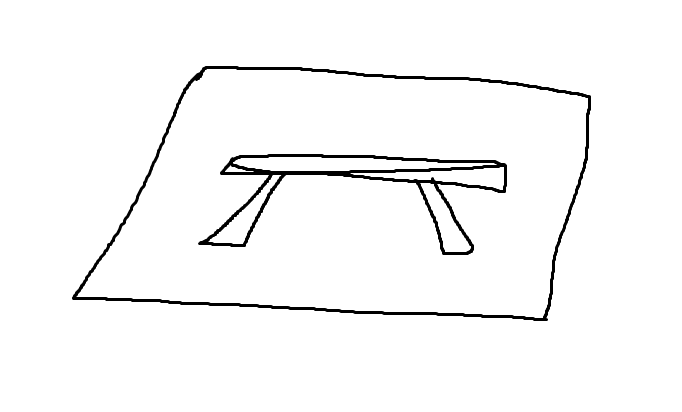
\includegraphics[width=\linewidth]{pics/bildverarbeitungsalgos/ApproxPolyDP_input.png}
        \caption{Input}
        \label{maai:wrapperspective:input}
    \end{minipage}
    \hfill
    \begin{minipage}[t]{0.45\linewidth}
        \centering
        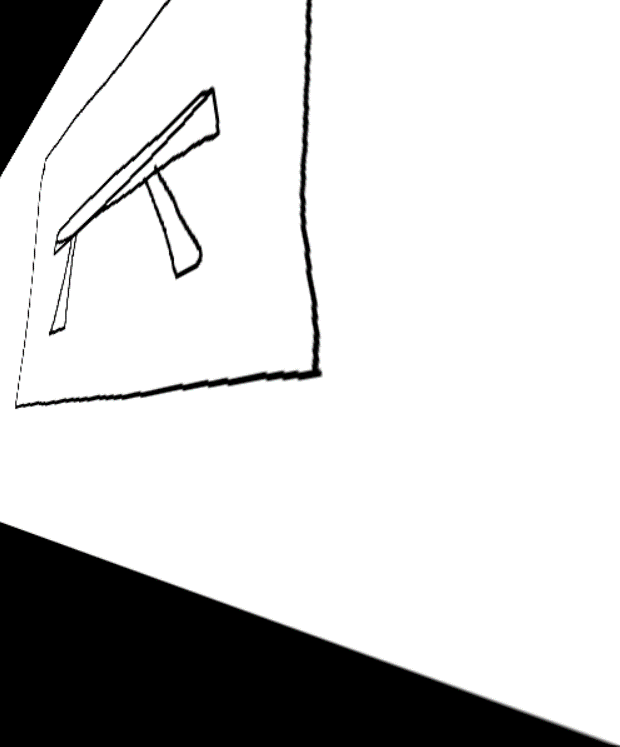
\includegraphics[width=\linewidth]{pics/bildverarbeitungsalgos/wrapperspective.png}
        \caption{perspektiventransformiert}
        \label{maai:wrapperspective:output}
    \end{minipage}
\end{figure}

\subsubsection{Umwandlung der Bilder in für das Spiel brauchbare Daten [H]}
Hat man nun das Bild Perspektiven transformiert, so kann man dies mit dem Send-Button (Wie in Abbildung \ref{fig:map:maperkennungsprozess} ersichtlich) bestätigen.
Somit wird das Bild an den Python-Server ein letztes Mal zurückgesendet und es wird eine spielbare Map daraus generiert.
Wie dies Funktioniert wird in den folgenden Codeblöcken ersichtlich.

Zuerst wird sich wieder darum gekümmert, dass die Daten so stark minimiert werden, dass sie trotzdem noch brauchbar sind, aber so viel wie möglich Informationen beinhalten. Das heißt: so wenig wie möglich Bildmaterial soll so viel wie möglich Information enthalten. Doch davor wird das übergebene Bild in den RGBA-Farbraum umgewandelt und in ein OpenCV2-Bild konvertiert. Im RGBA Farbraum ist es zusätzlich noch möglich neben den Farbwerten auch Informationen über die Transparenz des Bildes abzuspeichern. Dann startet wieder dasselbe Prozedere, wie bei der Perspektiven Transformation.

Zuerst wird das Bild in Graustufen konvertiert. Wie dies funktioniert ist bereits im Unterpunkt \ref{maai:grayscale} erklärt. Dann wird es unscharf gezeichnet und danach ein adaptiver Threshold (ein Schwellwert-Bild) daraus generiert.

Im nächsten Schritt wird die vorgefertigte Funktion ``Bitwise\_not'' angewendet. Hier wird das Bild in nur schwarze und weiße Pixel umgewandelt. Sie wandelt also alle Pixel entweder in schwarze oder weiße Bildpunkte um und generiert daraus wieder ein neues OpenCV2 Bild. Auch dieses Bild wird wieder unscharf gezeichnet.

Was dann noch für das Spiel wichtig ist, ist, dass das Bild in einen Quader umgewandelt wird. Das heißt, dass das Schwellwert-Bild so umgewandelt wird, dass alle Seiten (Höhe und Breite) gleich lang sind. Die leeren Flächen, die daraus entstehen werden mit transparenten Pixeln gefüllt.

Die Zeile zwanzig dient dazu das Bild testweise in einem Ordner abzuspeichern.

\begin{lstlisting}[language=Python,caption=Bild in Spielbare Map umwandeln,label=lst:umsetzung:getplayablearray]
    def getPlayableArray(img):
        np.set_printoptions(threshold=sys.maxsize)

        alpha_img = cv2.cvtColor(img, cv2.COLOR_BGR2BGRA)  # rgba
        imgWarpGray = cv2.cvtColor(alpha_img, cv2.COLOR_BGR2GRAY)
        blurred = cv2.GaussianBlur(imgWarpGray, (7, 7), 0)
        imgAdaptiveThre = cv2.adaptiveThreshold(
            blurred, 255, cv2.ADAPTIVE_THRESH_GAUSSIAN_C, cv2.THRESH_BINARY_INV, 7, 2)
        imgAdaptiveThre = cv2.bitwise_not(imgAdaptiveThre)
        imgAdaptiveThre = cv2.medianBlur(imgAdaptiveThre, 3)

        # make image square
        imgAdaptiveThre = np.array(makeSquare(
            cv2.cvtColor(imgAdaptiveThre, cv2.COLOR_BGR2BGRA)))

        img = cv2.cvtColor(imgAdaptiveThre, cv2.COLOR_BGR2BGRA)

        # pippoRGBA2 = Image.fromarray(np.array(img).astype('uint8'), mode='RGBA')
        # pippoRGBA2.show()
        cv2.imwrite('./source/prototypes/streamFusion/output/imgAdaptiveThre.png', imgAdaptiveThre)
\end{lstlisting}

Im nächsten Schritt wird der Array berechnet, welcher als Grundlage für die spielbare Map dient und aus dem aufgenommenen Bild extrahiert wird. Der Array beinhaltet nach der Verarbeitung schwarze und transparente Bildpunkte. Die schwarzen Pixel symbolisieren jene Plätze, auf welchen sich der Spieler schlussendlich bewegen kann. Die transparenten Pixel sind jene, welche als Hintergrund erkannt wurden und somit nicht für den Spieler begehbar sein sollten. Wie sich jedoch der Spieler auf diesen Punkten bewegen kann und wie der Array in die Spiellogik implementiert wird, wird im Kapitel ``Erstellung der Spielumgebung \ref {impl:Spielumgebung}'' von Rafetseder Tobias näher erklärt.

Jedoch wird zuerst eben das transformierte Bild in den Array umgewandelt. Dafür wird aus diesem adaptiven Threshold-Bild (Schwellwert-Bild) ein Faktor ausgerechnet, mit welchem die Bildpunkte zusammengefasst werden müssen, um insgesamt nicht mehr als \(\approx\)3025 Pixel zu überschreiten. Die dabei verwendete Formel wird im Folgenden an einem einfachen Beispiel erklärt. Diese lautet:

\[
    n \approx math.ceil(\sqrt{ \frac{ rows * columns }{ meshes } })
\]

Setzt man nun eine Bildbreite und eine Bildhöhe in ``rows'' und ``columns'' ein, so erhält man den ganzzahligen Faktor, mit welchem die angegebene Bildbreite und Höhe multipliziert werden muss, um maximal \(\approx\)3025 Pixel zu erreichen.
Angenommen also, das Bild ist 1920x1080 Pixel groß, so würde das eine Anzahl von 2.073.600 Pixel liefer. Setzt man diese Werte nun in die Formel ein, so erhält man den Faktor 27. Dividiert man nun die beiden Bildmaße mit diesem Wert, so erhält man ein Bild, welches 72x40 groß ist und somit eine Anzahl von 2880 Pixel liefert und somit weit unter den geforderten 3025 Pixeln liegt.

Der Grund, warum der Array eine maximale Größe von 3025 Einträgen hat, ist, weil p5.js, die Bibliothek, welche wir verwenden, um die Spielumgebung aufzubauen nur ein Maximum von 1000 Meshes generieren kann, bevor das Spiel zu ruckeln beginnt. Und wir gehen davon aus, dass man nie mehr als ein Drittel seines Blattes vollzeichnen wird.

Dann wird in einer zweidimensionalen Schleife das Bild durchgegangen und jeweils alle n Pixel ein Mittelwert errechnen über die Farbwerte des Bildes errechnet und somit der Hintergrund vom Vordergrund getrennt. Alle n Pixel werden zusammengefasst. Wenn in diesem Code also mehr als 95\% der Pixel Hintergrund darstellen, so wird der Pixel auch als Hintergrund gewertet (es wird also in den Map-Array ein transparenter Pixel an der Stelle x/n und y/n gepusht). Ansonsten wird ein Schwarzer Pixel (als Map erkannt) dem Map-Array hinzugefügt. An dem Punkt mit den Koordinaten x/n und y/n befindet sich also der neue Bildpunkt, da das Bild ja komprimiert werden soll.

Dieser Map-Array wird dann in ein File abgespeichert. Dieses File dient rein dazu, um den Array debuggen zu können. Darunter wird ein Bild, welches aus diesem Map-Array generiert worden ist, im angegebenen Pfad gespeichert.

\begin{lstlisting}[language=Python,label=lst:umsetzung:getArray,firstnumber=21]
        iar = np.asarray(img).tolist()

        rows = len(iar)
        columns = len(iar[0])

        meshes = 3025
        # percent = perc(rows * columns)
        percent = 95
        n = math.ceil(np.sqrt(rows * columns / meshes))
        x = 0
        y = 0

        newImg = []

        while y < rows:
            newImg.append([])
            while x < columns:

                i = 0
                j = 0
                bg = 0
                while i < n:
                    while j < n:
                        if (y + j) < rows and (x + i) < columns:
                            if np.all(iar[y + j][x + i][:3] == [255, 255, 255], 0):
                                bg += 1
                        else:
                            bg += 1
                        j += 1
                    j = 0
                    i += 1

                bgPercent = bg / (n**2)
                if (bgPercent < (percent / 100)):
                    newImg[int(y / n)].append([0, 0, 0, 255])
                else:
                    newImg[int(y / n)].append([255, 255, 255, 0])

                x += n
            x = 0
            y += n

        iar = np.asarray(newImg).tolist()
        with open('./source/prototypes/streamFusion/output/mapArray.txt', 'w') as f:
            f.writelines(repr(iar))

        # pippoRGBA2 = Image.fromarray(np.array(newImg).astype('uint8'), mode='RGBA')
        # pippoRGBA2.show()
        cv2.imwrite(
            './source/prototypes/streamFusion/output/newImg.png', np.array(newImg))

        return newImg

\end{lstlisting}

\subsection{Kommunikation mit der Lobby via Flask und Flask SocketIO [W]}

\section{KI [H]}\label{maai:ai:title}

Die Vorstellung von Künstlichen Intelligenzen gibt es schon seit Mitte des zwanzigsten Jahrhunderts. Bei einer Konferenz von Wissenschaftlern am Dartmouth College im US-Bundesstaat New Hampshire im Jahr 1956 wird das erste Mal bewiesen, dass es möglich ist mit Mathematik menschliche Intelligenz zu simulieren.

%Quelle: https://www.bosch.com/de/stories/geschichte-der-kuenstlichen-intelligenz/
Der Gedanke, dass eine von Menschenhand erschaffene Intelligenz, welche keine biologische Abstammung hat und den Menschen bei der Arbeit unterstützen, oder diese ganz abnehmen kann, wird seit diesem Ereignis angestrebt. Dabei ist das Feld, in welchem ``Artificial Intelligence'' (AI) beziehungsweise Künstliche Intelligenz (KI) eingesetzt werden kann, scheinbar unbegrenzt.

Das Einzige, das gegeben sein muss, ist, dass in einem komplexen System, in welcher die Künstliche Intelligenz operiert, Daten extrahiert und gesammelt werden können. Weiters sind Ressourcen, wie Hardware oder Zeit, ein wichtiger Aspekt. Die intelligente Maschine kann mehrere Millionen Schritte pro Tag ausführen und mit mehreren ``Gehirnen'' (Mehrere Instanzen der des Lernumfelds) gleichzeitig lernen. Trotzdem ist dies limitiert, durch die Geschwindigkeit und der Rechenleistung, die zu diesem Zeitpunkt aufgebracht werden kann, mit welcher die Aktionen ausgeführt werden und somit zu einem ``Lernen'' führen.

Die zuvor genannte ``Lern-Technik'' Reinforcementlearning (Kapitel \ref{}), funktioniert ähnlich wie die Lern-Art von biologischen Organismen. Die Idee stammt davon, dass simple, Lebensformen, welche nicht mehr als Instinkte zum Futter sammeln, Prädatoren ausweichen und im Generellen zum Überleben haben, sollten von einer Maschine ``leicht'' simuliert werden können. Ein Beispiel hierfür wäre ein Fadenwurm. Das ZNS (Zentrale Nervensystem) baut sich aus dreihundertzwei Nervenzellen zusammen. Weitere chemische Verbindungsstellen und Kanäle erhöhen die Komplexität dieses Lebewesens nur wenig. Dies ist mit modernen Computern bereits simulierbar.
%Quelle: https://www.sueddeutsche.de/wissen/gehirngroesse-von-0-bis-11-000-000-000-neuronen-1.1850384

Dazu müssen jedoch gewisse mathematische Modelle angewandt werden, um dieses Ergebnis zu erreichen und den Organismus zu simulieren.

Dass und wie es für eine Maschine möglich ist zu lernen wurde bereits im Kapitel \ref {tech:ki:head} näher erläutert.

Um diese mathematischen Modelle jedoch perfekt auf ein gewünschtes Ergebnis abstimmen zu können, wir Hpyerparamter-``Fine-Tuning'' angewendet. Dabei werden jene Parameter, welche zu einem Lernen beitragen, so angepasst, dass das Modell eine perfekte Lernkurve erzielt.

Im Zuge dieser Arbeit wurde klar, dass Künstliche Intelligenz kein Thema ist, welches leicht zu begreifen ist.

Diese zuvor erwähnten mathematischen Modelle wurden bereits in einer Python Bibliothek namens ``Stable\_baselines3'' implementiert. Dieses Framework wird im Folgenden (Kapitel: \ref {maai:usedLibraries}) genauer erklärt.

Die zur Verfügung gestellten Algorithmen sind jedoch nicht perfekt auf unseren Anwendungsfall abgestimmt. Trotzdem wurden Ergebnisse erzielt (auch, wenn diese nicht bemerkenswert sind).

Die Logik der Welt, in welcher sich der Agent (Reinforcement-Learning) bewegt, wurde mittels Open-AI-Gym umgesetzt. Dabei handelt es sich um eine Hilfestellung, welche es ermöglicht objektorientiert eine Künstliche Intelligenz mit Python umzusetzen. Die Syntax beziehungsweise Vorgehensweise, welche verwendet wird, um eine Künstliche Intelligenz, welche mit der Methode des verstärkten Lernens trainiert, mittels Python zu implementieren, wird in den folgenden Kapiteln genauer beschrieben. Dabei wird auch genauer auf die genannten Bibliotheken eingegangen.

\subsection{Verwendete Bibliotheken [H]}\label{maai:usedLibraries}


syntax (gym.make(), obs, step, und so zeig)

% \subsection{Künstliche Intelligenz Definition [H]}
\subsection{Reinforcement Learning [H]}
Code
Wie wurde reward vergeben
\subsection{Die ScribbleFight-KI [H]}\label{maai:scribblefightki}

Im Laufe der Ausarbeitung der Diplomarbeit und der damit zusammenhängenden Forschung änderte sich oft die
Vorstellung darüber, wie das Endprodukt (KI) auszusehen hat, beziehungsweise, wie dieses aussehen kann.
Limitierungen, welche vor der Forschung noch nicht bekannt und bewusst waren, begrenzten die Lernfähigkeit der KI.
Auf Probleme, Lösungen und Ergebnisse wird jedoch noch näher in \ref{maai:scribblefightki} eingegangen.


Ziele
Umsetzung
code (eher so vom rafi)
\subsubsection{Beschreibung der Funktionalität [H]}
Was sieht die KI?
\begin{figure}[H]
    \centering
    \begin{minipage}[t]{0.45\linewidth}
        \centering
        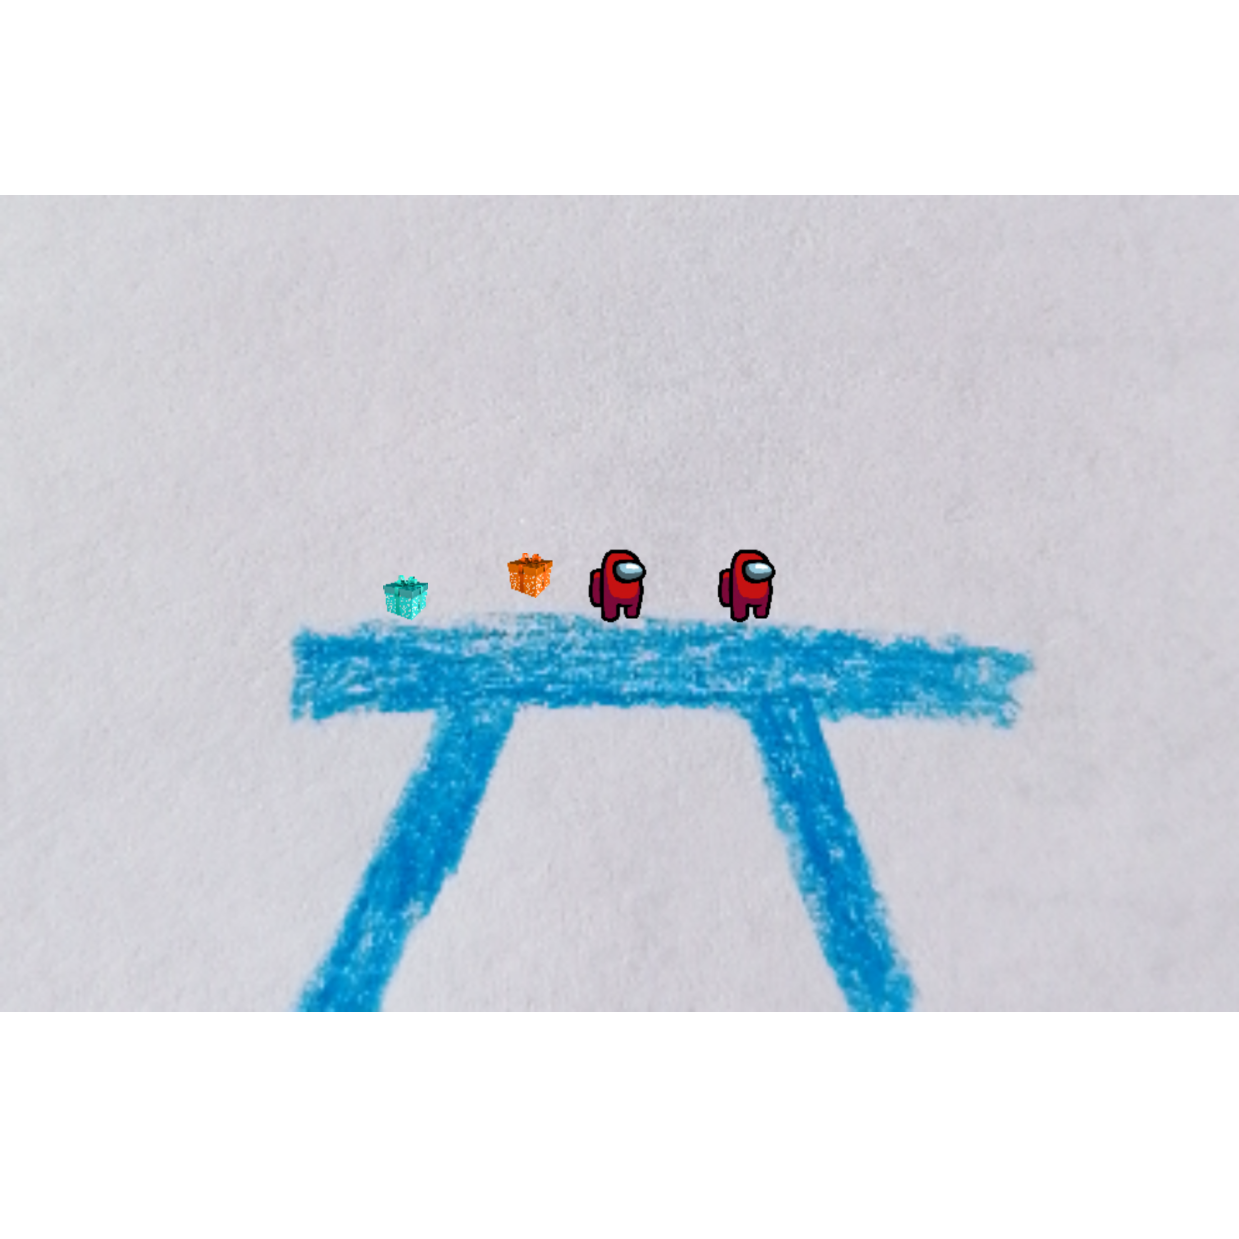
\includegraphics[width=\linewidth]{pics/ai/screenshots.png}
        \caption{Spieler Sicht}
        \label{maai:ai:visCopy:input}
    \end{minipage}
    \hfill
    \begin{minipage}[t]{0.45\linewidth}
        \centering
        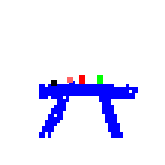
\includegraphics[width=\linewidth]{pics/ai/newImg.png}
        \caption{KI Sicht}
        \label{maai:ai:visCopy:output}
    \end{minipage}
\end{figure}
\subsubsection{Warum Python? [H]}
% \subsection{Tensorflow und Keras [H]}
% \subsubsection{Tensorflow [H]}
% \subsubsection{Keras [H]}
